\chapter{Batch effects and the effective design of single-cell gene expression studies}

Single-cell RNA sequencing (scRNA-seq) can be used to characterize
variation in gene expression levels at high resolution. However, the
sources of experimental noise in scRNA-seq are not yet well understood.
We investigated the technical variation associated with sample
processing using the single-cell Fluidigm C1 platform. To do so, we
processed three C1 replicates from three human induced pluripotent stem
cell (iPSC) lines. We added unique molecular identifiers (UMIs) to all
samples, to account for amplification bias. We found that the major
source of variation in the gene expression data was driven by genotype,
but we also observed substantial variation between the technical
replicates. We observed that the conversion of reads to molecules using
the UMIs was impacted by both biological and technical variation,
indicating that UMI counts are not an unbiased estimator of gene
expression levels. Based on our results, we suggest a framework for
effective scRNA-seq studies.

\section{Introduction}\label{introduction}

Single-cell genomic technologies can be used to study the regulation of
gene expression at unprecedented resolution \citep{Macaulay2014,
Saliba2014}. Using single-cell gene expression data, we can begin to
effectively characterize and classify individual cell types and cell
states, develop a better understanding of gene regulatory threshold
effects in response to treatments or stress, and address a large number
of outstanding questions that pertain to the regulation of noise and
robustness of gene expression programs. Indeed, single cell gene
expression data have already been used to study and provide unique
insight into a wide range of research topics, including differentiation
and tissue development \citep{Macosko2015, Handel2016, Drissen2016},
the innate immune response \citep{Shalek2013, Jaitin2014}, and
pharmacogenomics \citep{Miyamoto2015, Kim2015}.

Yet, there are a number of outstanding challenges that arose in parallel
with the application of single cell technology \citep{Stegle2015}. A
fundamental difficulty, for instance, is the presence of inevitable
technical variability introduced during sample processing steps,
including but not limited to the conditions of mRNA capture from a
single cell, amplification bias, sequencing depth, and variation in
pipetting accuracy. These (and other sources of error) may not be unique
to single cell technologies, but in the context of studies where each
sample corresponds to a single cell, and is thus processed as a single
unrepeatable batch, these technical considerations make the analysis of
biological variability across single cells particularly challenging.

To better account for technical variability in scRNA-seq experiments, it
has become common to add spike-in RNA standards of known abundance to
the endogenous samples \citep{Brennecke2013, Grun2014}. The most
commonly used spike-in was developed by the External RNA Controls
Consortium (ERCC) \citep{Jiang2011}; comprising of a set of 96 RNA
controls of varying length and GC content. A number of single cell
studies focusing on analyzing technical variability based on ERCC
spike-in controls have been reported \citep{Brennecke2013, Grun2014,
Ding2015, Vallejos2015}. However, one principle problem with
spike-ins is that they do not `experience' all processing steps that the
endogenous sample is subjected to. For that reason, it is unknown to
what extent the spike-ins can faithfully reflect the error that is being
accumulated during the entire sample processing procedure, either within
or across batches. In particular, amplification bias, which is assumed
to be gene-specific, cannot be addressed by spike-in normalization
approaches.

To address challenges related to the efficiency and uniformity with
which mRNA molecules are amplified and sequenced in single cells, unique
molecule identifiers (UMIs) were introduced to single cell sample
processing \citep{Kivioja2011, Fu2011, Casbon2011, Shiroguchi2012}.
The rationale is that by counting molecules rather than the number of
amplified sequencing reads, one can account for biases related to
amplification, and obtain more accurate estimates of gene expression
levels \citep{Jaitin2014, Islam2014, Grun2014}. It is assumed that most
sources of variation in single cell gene expression studies can be
accounted for by using the combination of UMIs and a spike-in based
standardization \citep{Islam2014, Vallejos2015}. Nevertheless, though
molecule counts, as opposed to sequencing read counts, are associated
with substantially reduced levels of technical variability, a
non-negligible proportion of experimental error remains unexplained.

There are a few common platforms in use for scRNA-seq. The automated C1
microfluidic platform (Fluidigm), while more expensive per sample, has
been shown to confer several advantages over platforms that make use of
droplets to capture single cells \citep{Wu2014, Macosko2015}. In
particular, smaller samples can be processed using the C1 (when cell
numbers are limiting), and the C1 capture efficiency of genes (and RNA
molecules) is markedly higher. Notably, in the context of this study,
the C1 system also allows for direct confirmation of single cell capture
events, in contrast to most other microfluidic-based approaches
\citep{Macosko2015, Klein2015}. One of the biggest limitations of using
the C1 system, however, is that single cell capture and preparation from
different conditions are fully independent \citep{Hicks2015}.
Consequently, multiple replicates of C1 collections from the same
biological condition are necessary to facilitate estimation of technical
variability even with the presence of ERCC spike-in controls
\citep{Stegle2015}. To our knowledge, to date, no study has been
purposely conducted to assess the technical variability across batches
on the C1 platform.

To address this gap, we collected scRNA-seq data from induced
pluripotent stem cell (iPSC) lines of three Yoruba individuals
(abbreviation: YRI) using C1 microfluidic plates. Specifically, we
performed three independent C1 collections per each individual to
disentangle batch effects from the biological covariate of interest,
which, in this case, is the difference between individuals. Both ERCC
spike-in controls and UMIs were included in our sample processing. With
these data, we were able to elucidate technical variability both within
and between C1 batches and thus provide a deep characterization of
cell-to-cell variation in gene expression levels across individuals.

\section{Results}\label{results}

\subsection{Study design and quality
control}\label{study-design-and-quality-control}

We collected single cell RNA-seq (scRNA-seq) data from three YRI iPSC
lines using the Fluidigm C1 microfluidic system followed by sequencing.
We added ERCC spike-in controls to each sample, and used 5-bp random
sequence UMIs to allow for the direct quantification of mRNA molecule
numbers. For each of the YRI lines, we performed three independent C1
collections; each replicate was accompanied by processing of a matching
bulk sample using the same reagents. This study design (Fig. 1A and
Supplementary Table S1) allows us to estimate error and variability
associated with the technical processing of the samples, independently
from the biological variation across single cells of different
individuals. We were also able to estimate how well scRNA-seq data can
recapitulate the RNA-seq results from population bulk samples.

\begin{figure}[htbp]
\centering
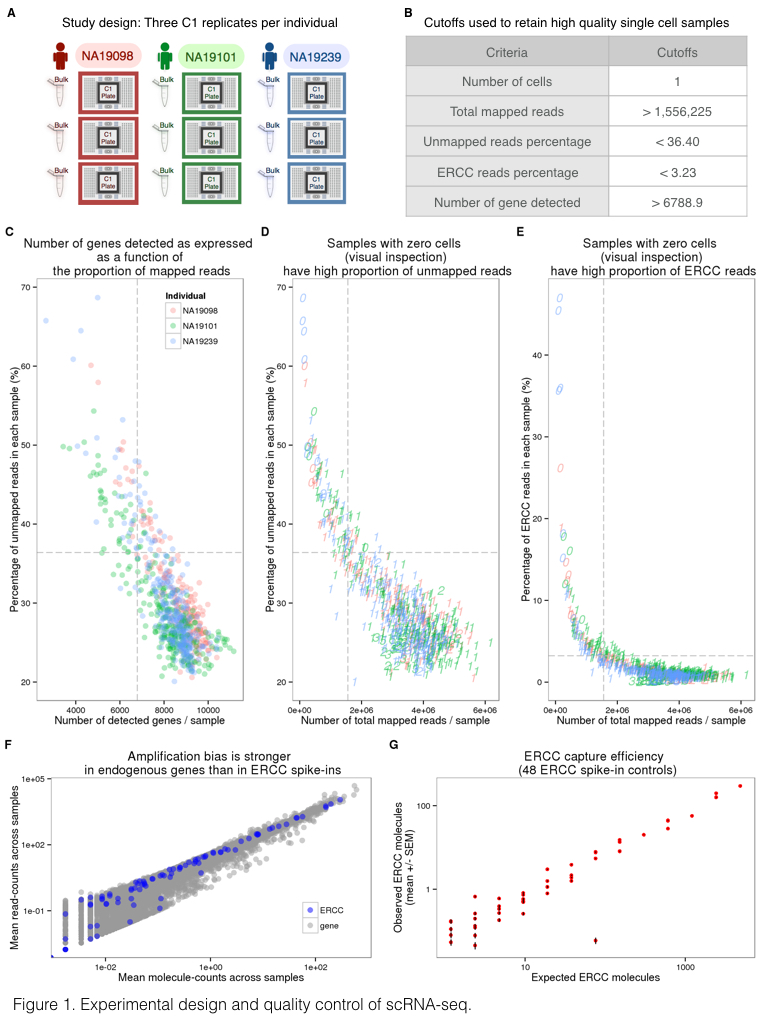
\includegraphics[trim=0 .5in 0 0,clip,width=5in]{img/ch04/Figure01.jpeg}
\caption{\textbf{Figure 1. Experimental design and quality control of
scRNA-seq.} (A) Three C1 96 well-integrated fluidic circuit (IFC)
replicates were collected from each of the three Yoruba individuals. A
bulk sample was included in each batch. (B) Summary of the cutoffs used
to remove data from low quality cells that might be ruptured or dead
(See Supplementary Fig. S1 for details). (C-E) To assess the quality of
the scRNA-seq data, the capture efficiency of cells and the faithfulness
of mRNA fraction amplification were determined based on the proportion
of unmapped reads, the number of detected genes, the numbers of total
mapped reads, and the proportion of ERCC spike-in reads across cells.
The dash lines indicate the cutoffs summarized in panel (B). The three
colors represent the three individuals (NA19098 in red, NA19101 in
green, and NA19239 in blue), and the numbers indicate the cell numbers
observed in each capture site on C1 plate. (F) Scatterplots in log scale
showing the mean read counts and the mean molecule counts of each
endogenous gene (grey) and ERCC spike-ins (blue) from the 564 high
quality single cell samples before removal of genes with low expression.
(G) mRNA capture efficiency shown as observed molecule count versus
number of molecules added to each sample, only including the 48 ERCC
spike-in controls remaining after removal of genes with low abundance.
Each red dot represents the mean +/- SEM of an ERCC spike-in across the
564 high quality single cell samples.}
\end{figure}

In what follows, we describe data as originating from different samples
when we refer to data from distinct wells of each C1 collection.
Generally, each sample corresponds to a single cell. In turn, we
describe data as originating from different replicates when we refer to
all samples from a given C1 collection, and from different individuals
when we refer to data from all samples and replicates of a given
genetically distinct iPSC line.

We obtained an average of 6.3 +/- 2.1 million sequencing reads per
sample (range 0.4-11.2 million reads). We processed the sequencing reads
using a standard alignment approach (see Methods) and performed multiple
quality control analyses. As a first step, we estimated the proportion
of ERCC spike-in reads from each sample. We found that, across samples,
sequencing reads from practically all samples of the second replicate of
individual NA19098 included unusually high ERCC content compared to all
other samples and replicates (Supplementary Fig. S1). We concluded that
a pipetting error led to excess ERCC content in this replicate and we
excluded the data from all samples of this replicate in subsequent
analyses. With the exception of the excluded samples, data from all
other replicates seem to have similar global properties (using general
metrics; Fig. 1C-E and Supplementary Fig. S1).

We next examined the assumption that data from each sample correspond to
data from a single cell. After the cell sorting was complete, but before
the processing of the samples, we performed visual inspection of the C1
microfluidic plates. Based on that visual inspection, we flagged 21
samples that did not contain any cell, and 54 samples that contained
more than one cell (across all batches). Visual inspection of the C1
microfluidic plate is an important quality control step, but it is not
infallible. We therefore filtered data from the remaining samples based
on the number of total mapped reads, the percentage of unmapped reads,
the percentage of ERCC spike-in reads, and the number of genes detected
(Fig. 1B-E). We chose data-driven inclusion cutoffs for each metric,
based on the 95th percentile of the respective distributions for the 21
libraries that were amplified from samples that did not include a cell
based on visual inspection (Supplementary Fig. S1). Using this approach,
we identified and removed data from 15 additional samples that were
classified as originating from a single cell based on visual inspection,
but whose data were more consistent with a multiple-cell origin based on
the number of total molecules, the concentration of cDNA amplicons, and
the read-to-molecule conversion efficiency (defined as the number of
total molecules divided by the number of total reads; Supplementary Fig.
S2). At the conclusion of these quality control analyses and exclusion
steps, we retained data from 564 high quality samples, which correspond,
with reasonable confidence, to 564 single cells, across eight replicates
from three individuals (Supplementary Table S2).

Our final quality check focused on the different properties of
sequencing read and molecule count data. We considered data from the 564
high quality samples and compared gene specific counts of sequencing
read and molecules. We found that while gene-specific reads and molecule
counts are exceptionally highly correlated when we considered the ERCC
spike-in data (r = 0.99; Fig. 1F), these counts are somewhat less
correlated when data from the endogenous genes are considered (r =
0.92). Moreover, the gene-specific read and molecule counts correlation
is noticeably lower for genes that are expressed at lower levels (Fig.
1F). These observations concur with previous studies \citep{Islam2014,
Grun2014} as they underscore the importance of using UMIs in single
cell gene expression studies.

\begin{figure}[htbp]
\centering
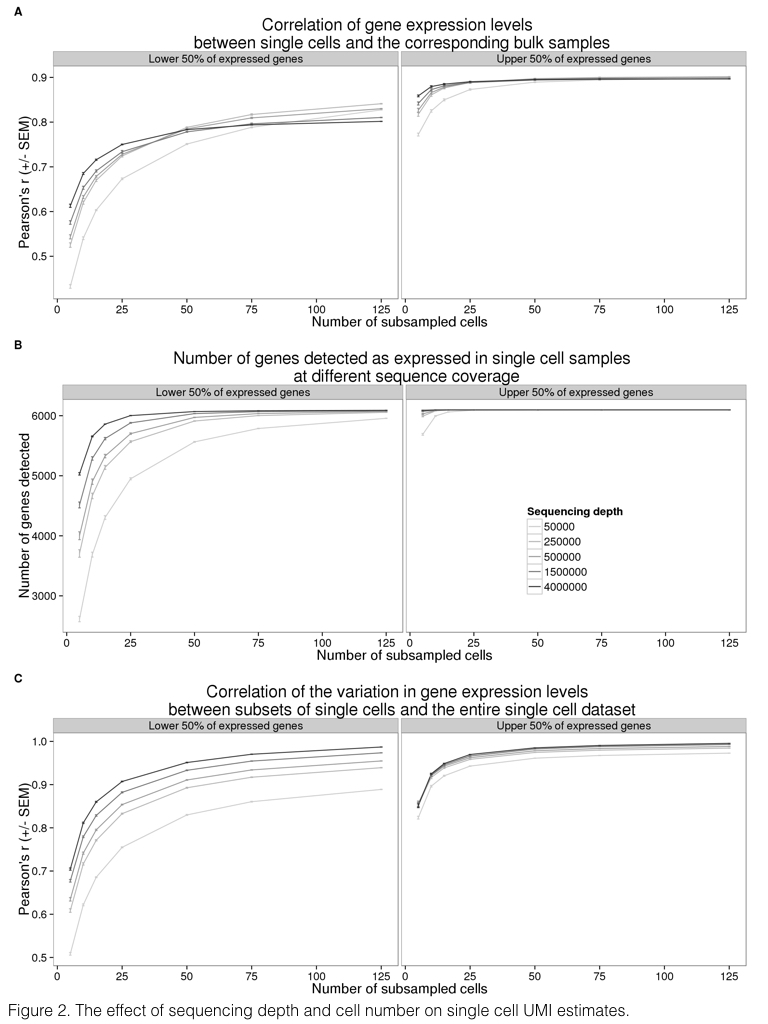
\includegraphics[trim=0 .3in 0 0,clip,width=5in]{img/ch04/Figure02.jpeg}
\caption{\textbf{Figure 2. The effect of sequencing depth and cell
number on single cell UMI estimates.} Sequencing reads from the entire
data set were subsampled to the indicated sequencing depth and cell
number, and subsequently converted to molecules using the UMIs. Each
point represents the mean +/- SEM of 10 random draws of the indicated
cell number. The left panel displays the results for 6,097 (50\% of
detected) genes with lower expression levels and the right panel the
results for 6,097 genes with higher expression levels. (A) Pearson
correlation of aggregated gene expression level estimates from single
cells compared to the bulk sequencing samples. (B) Total number of genes
detected with at least one molecule in at least one of the single cells.
(C) Pearson correlation of cell-to-cell gene expression variance
estimates from subsets of single cells compared to the full single cell
data set.}
\end{figure}

We proceeded by investigating the effect of sequencing depth and the
number of single cells collected on multiple properties of the data. To
this end, we repeatedly subsampled single cells and sequencing reads to
assess the correlation of the single cell gene expression estimates to
the bulk samples, the number of genes detected, and the correlation of
the cell-to-cell gene expression variance estimates between the reduced
subsampled data and the full single cell gene expression data set (Fig.
2). We observed quickly diminishing improvement in all three properties
with increasing sequencing depth and the number of sampled cells,
especially for highly expressed genes. For example, a per cell
sequencing depth of 1.5 million reads (which corresponds to
\textasciitilde{}50,000 molecules) from each of 75 single cells was
sufficient for effectively quantifying even the lower 50\% of expressed
genes. At this level of subsampling for individual NA19239, we were able
to detect a mean of 6068 genes out of 6097 genes expressed in the bulk
samples (the bottom 50\%; Fig. 2B); the estimated single cell expression
levels of these genes (summed across all cells) correlated with the bulk
sample gene expression levels with a mean Pearson coefficient of 0.8
(Fig. 2A), and the estimated cell-to-cell variation in gene expression
levels was correlated with the variation estimated from the full data
set with a mean Pearson coefficient of 0.95 (Fig. 2C).

\subsection{Batch effects associated with UMI-based single cell
data}\label{batch-effects-associated-with-umi-based-single-cell-data}

In the context of the C1 platform, typical study designs make use of a
single C1 plate (batch/replicate) per biological condition. In that
case, it is impossible to distinguish between biological and technical
effects associated with the independent capturing and sequencing of each
C1 replicate. We designed our study with multiple technical replicates
per biological condition (individual) in order to directly and
explicitly estimate the batch effect associated with independent C1
preparations (Fig. 1A).

As a first step in exploring batch effects, we examined the gene
expression profiles across all single cells that passed our quality
checks (as reported above) using raw molecule counts (without
standardization). Using principal component analysis (PCA) for
visualization, we observed -- as expected - that the major source of
variation in data from single cells is the individual origin of the
sample (Fig. 4A). Specifically, we found that the proportion of variance
due to individual was larger (median: 8\%) than variance due to C1 batch
(median: 4\%; Kruskal-Wallis test; \emph{P} \textless{} 0.001,
Supplementary Fig. S3; see Methods for details of the variance component
analysis). Yet, variation due to C1 batch is also substantial - data
from single cell samples within a batch are more correlated than that
from single cells from the same individual but different batches
(Kruskal-Wallis test; \emph{P} \textless{} 0.001).

Could we account for the observed batch effects using the ERCC spike-in
controls? In theory, if the total ERCC molecule-counts are affected only
by technical variability, the spike-ins could be used to correct for
batch effects even in a study design that entirely confounds biological
samples with C1 preparations. To examine this, we first considered the
relationship between total ERCC molecule-counts and total endogenous
molecule-counts per sample. If only technical variability affects ERCC
molecule-counts, we expect the technical variation in the spike-ins
(namely, variation between C1 batches) to be consistent, regardless of
the individual assignment. Indeed, we observed that total ERCC
molecule-counts are significantly different between C1 batches (F-test;
\emph{P} \textless{} 0.001). However, total ERCC molecule-counts are
also quite different across individuals, when variation between batches
is taken into account (LRT; \emph{P} = 0.08; Fig. 3A). This observation
suggests that both technical and biological variation affect total ERCC
molecule-counts. In addition, while we observed a positive relationship
between total ERCC molecule-counts and total endogenous molecule-counts
per sample, this correlation pattern differed across C1 batches and
across individuals (F-test; \emph{P} \textless{} 0.001; Fig. 3B).

To more carefully examine the technical and biological variation of ERCC
spike-in controls, we assessed the ERCC per-gene expression profile. We
observed that the ERCC gene expression data from samples of the same
batch were more correlated than data from samples across batches
(Kruskal-Wallis test; Chi-squared \emph{P} \textless{} 0.001). However,
the proportion of variance explained by the individual was significantly
larger than the variance due to C1 batch (median: 9\% vs.~5\%,
Chi-squared test; \emph{P} \textless{} 0.001, Supplementary Fig. S3),
lending further support to the notion that biological variation affects
the ERCC spike in data. Based on these analyses, we concluded that ERCC
spike-in controls cannot be used to effectively account for the batch
effect associated with independent C1 preparations.

\begin{figure}[htbp]
\centering
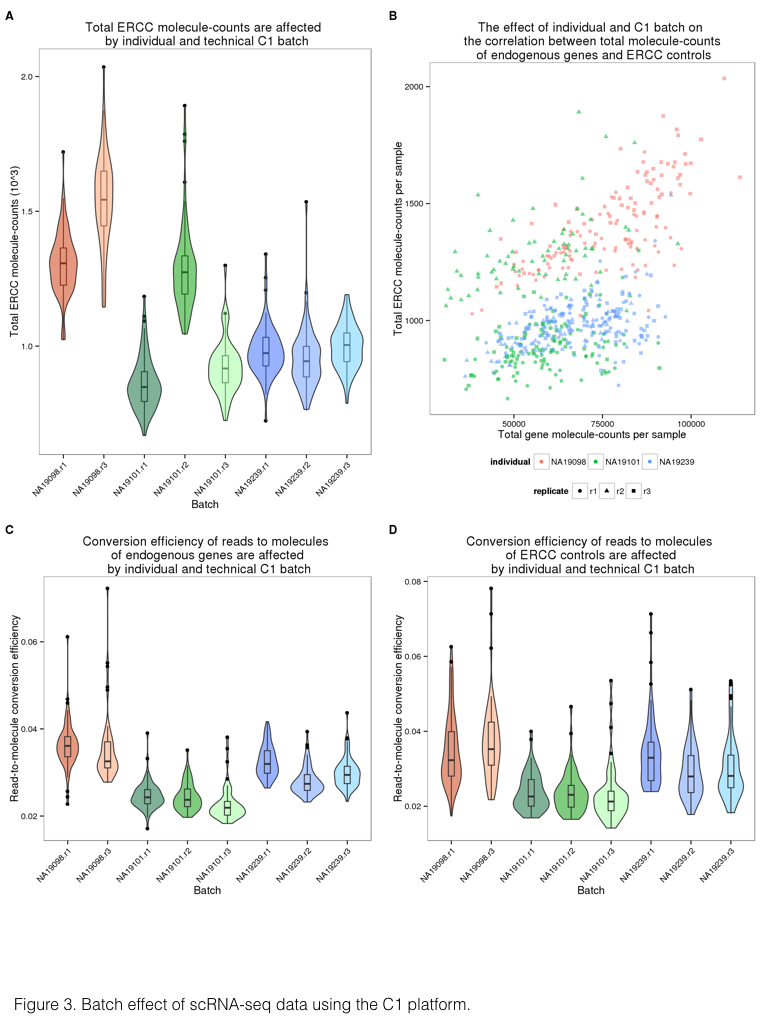
\includegraphics[trim=0 .5in 0 0,clip,width=5in]{img/ch04/Figure03.jpeg}
\caption{\textbf{Figure 3. Batch effect of scRNA-seq data using the C1
platform.} (A) Violin plots of the number of total ERCC spike-in
molecule-counts in single cell samples per C1 replicate. (B) Scatterplot
of the total ERCC molecule-counts and total gene molecule-counts. The
colors represent the three individuals (NA19098 is in red, NA19101 in
green, and NA19239 in blue). Data from different C1 replicates is
plotted in different shapes. (C and D) Violin plots of the reads to
molecule conversion efficiency (total molecule-counts divided by total
read-counts per single cells) by C1 replicate. The endogenous genes and
the ERCC spike-ins are shown separately in (C) and (D), respectively.
There is significant difference across individuals of both endogenous
genes (\emph{P} \textless{} 0.001) and ERCC spike-ins (\emph{P}
\textless{} 0.05). The differences across C1 replicates per individual
of endogenous genes and ERCC spike-ins were also evaluated (both
\emph{P} \textless{} 0.01).}
\end{figure}

We explored potential reasons for the observed batch effects, and in
particular, the difference in ERCC counts across batches and
individuals. We focused on the read-to-molecule conversion rates,
i.e.~the rates at which sequencing reads are converted to molecule
counts based on the UMI sequences. We defined read-to-molecule
conversion efficiency as the total molecule-counts divided by the total
reads-counts in each sample, considering separately the reads/molecules
that correspond to endogenous genes or ERCC spike-ins (Fig. 3C and 3D).
We observed a significant batch effect in the read-to-molecule
conversion efficiency of both ERCC (F-test; \emph{P} \textless{} 0.05)
and endogenous genes (F-test; \emph{P} \textless{} 0.001) across C1
replicates from the same individual. Moreover, the difference in
read-to-molecule conversion efficiency across the three individuals was
significant not only for endogenous genes (LRT; \emph{P} \textless{}
0.01, Fig. 3C) but also in the ERCC spike-ins (LRT; \emph{P} \textless{}
0.01, Fig. 3D). We reason that the difference in read to molecule
conversion efficiency across C1 preparations may contribute to the
observed batch effect in this platform.

\subsection{Measuring regulatory noise in single-cell gene expression
data}\label{measuring-regulatory-noise-in-single-cell-gene-expression-data}

Our analysis indicated that there is a considerable batch effect in the
single cell gene expression data collected from the C1 platform. We thus
sought an approach that would account for the batch effect and allow us
to study biological properties of the single-cell molecule count-based
estimates of gene expression levels, albeit in a small sample of just
three individuals. As a first step, we adjusted the raw molecule counts
by using a Poisson approximation to account for the random use of
identical UMI sequences in molecules from highly expressed genes (this
was previously termed a correction for the UMI `collision probability'
\citep{Fu2011}). We then excluded data from genes whose inferred molecule
count exceeded 1,024 (the theoretical number of UMI sequences) -- this
step resulted in the exclusion of data from 6 mitochondrial genes.

\begin{figure}[htbp]
\centering
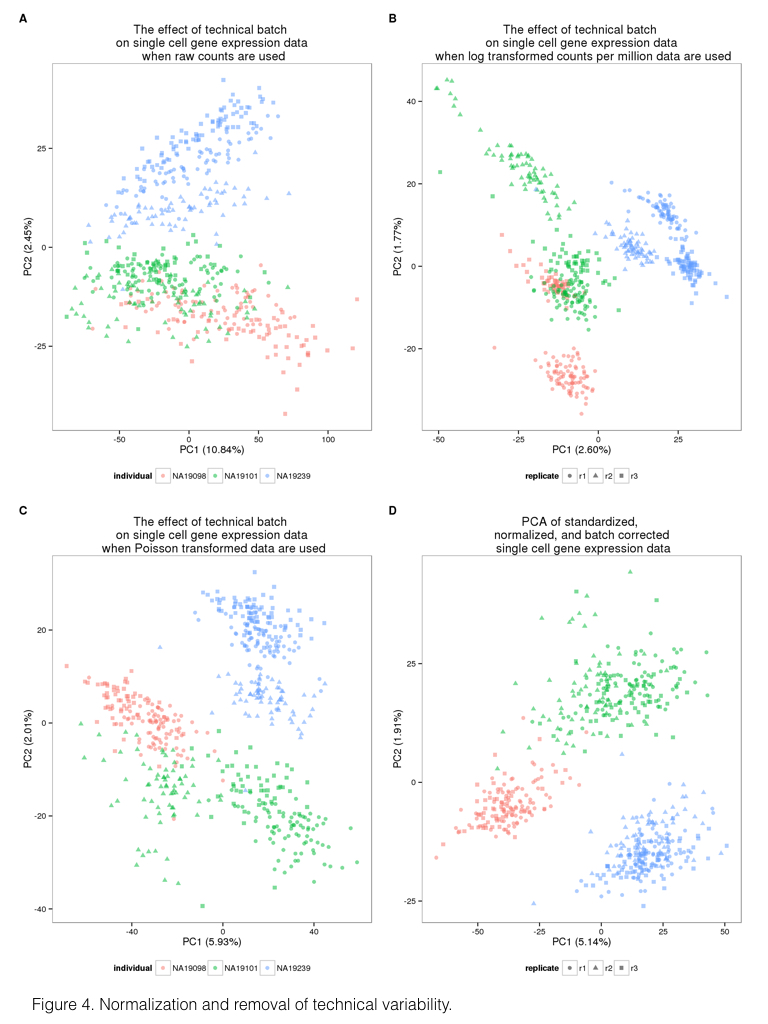
\includegraphics[trim=0 .5in 0 0,clip,width=5in]{img/ch04/Figure04.jpeg}
\caption{\textbf{Figure 4. Normalization and removal of technical
variability.} Principal component (PC) 1 versus PC2 of the (A) raw
molecule counts, (B) log\textsubscript{2} counts per million (cpm), (C)
Poisson transformed expression levels (accounting for technical
variability modeled by the ERCC spike-ins), and (D) batch-corrected
expression levels. The colors represent the three individuals (NA19098
in red, NA19101 in green, and NA19239 in blue). Data from different C1
replicates is plotted in different shapes.}
\end{figure}

We next incorporated a standardization step by computing log transformed
counts-per-million (cpm) to remove the effect of different sequencing
depths, as is the common practice for the analysis of bulk RNA-seq data
(Fig. 4A and 4B). We used a Poisson generalized linear model to
normalize the endogenous molecule log\textsubscript{2} cpm values by the
observed molecule counts of ERCC spike-ins across samples. While we do
not expect this step to account for the batch effect (as discussed
above), we reasoned that the spike-ins allow us to account for a subset
of technical differences between samples, for example, those that arise
from differences in RNA concentration (Fig. 4C).

Finally, to account for the technical batch effect, we modeled
between-sample correlations in gene expression within C1 replicates (see
Methods). Our approach is similar in principle to limma, which was
initially developed for adjusting within-replicate correlations in
microarray data \citep{Smyth2005}. We assume that samples within each C1
replicate share a component of technical variation, which is independent
of biological variation across individuals. We fit a linear mixed model
for each gene, which includes a fixed effect for individual and a random
effect for batch. The batch effect is specific to each C1 replicate, and
is independent of biological variation across individuals. We use this
approach to estimate and remove the batch effect associated with
different C1 preparations (Fig. 4D).

Once we removed the unwanted technical variability, we focused on
analyzing biological variation in gene expression between single cells.
Our goal was to identify inter-individual differences in the amount of
variation in gene expression levels across single cells, or in other
words, to identify differences between individuals in the amount of
regulatory noise \citep{Raser2005}. In this context, regulatory noise is
generally defined as the coefficient of variation (CV) of the gene
expression levels of single cells \citep{Fehrmann2013}. In the following,
we used the standardized, normalized, batch-corrected molecule count
gene expression data to estimate regulatory noise (Fig. 4D). To account
for heteroscedasticity from Poisson sampling, we adjusted the CV values
by the average gene-specific expression level across cells of the same
individual. The adjusted CV is robust both to differences in gene
expression levels, as well as to the proportion of gene dropouts in
single cells.

To investigate the effects of gene dropouts (the lack of molecule
representation of an expressed gene \citep{Brennecke2013, Shalek2013})
on our estimates of gene expression noise, we considered the association
between the proportion of cells in which a given gene is undetected
(namely, the gene-specific dropout rate), the average gene expression
level, and estimates of gene expression noise. Across all genes, the
median gene-specific dropout was 22 percent. We found significant
individual differences (LRT; \emph{P} \textless{}
10\textsuperscript{-5}) in gene-specific dropout rates between
individuals in more than 10\% (1,214 of 13,058) of expressed endogenous
genes. As expected, the expression levels, and the estimated variation
in expression levels across cells, are both associated with
gene-specific dropout rates (Supplementary Fig. S4). However,
importantly, adjusted CVs are not associated with dropout rates
(Spearman's correlation = 0.04; Supplementary Fig. S4), indicating that
adjusted CV measurements are not confounded by the dynamic range of
single-cell gene expression levels.

We thus estimated mean expression levels and regulatory noise (using
adjusted CV) for each gene, by either including (Fig. 5A) or excluding
(Fig. 5B) samples in which the gene was not detected/expressed. We first
focused on general trends in the data. We ranked genes in each
individual by their mean expression level as well as by their estimated
level of variation across single cells. When we considered samples in
which a gene was expressed, we found that 887 of the 1,000 most highly
expressed genes in each individual are common to all three individuals
(Fig. 5C). In contrast, only 103 of the 1,000 most highly variable
(noisy) genes in each individual were common to all three individuals
(Fig. 5D). We found similar results when we considered data from all
single cells, regardless of whether the gene was detected as expressed
(Fig. 5E and 5F).

Next, we identified genes whose estimated regulatory noise (based on the
adjusted CV) is significantly different between individuals. For the
purpose of this analysis, we only included data from cells in which the
gene was detected as expressed. Based on permutations (Supplementary
Fig. S5), we classified the estimates of regulatory noise of 560 genes
as significantly different across individuals (empirical \emph{P}
\textless{} .0001, Supplementary Fig. S6 for examples; Supplementary
Table S3 for gene list). These 560 genes are enriched for genes involved
in protein translation, protein disassembly, and various biosynthetic
processes (Supplementary Table S4). Interestingly, among the genes whose
regulatory noise estimates differ between individuals, we found two
pluripotency genes, \emph{KLF4} and \emph{DPPA2} (Supplementary Fig.
S7).

\begin{figure}[htbp]
\centering
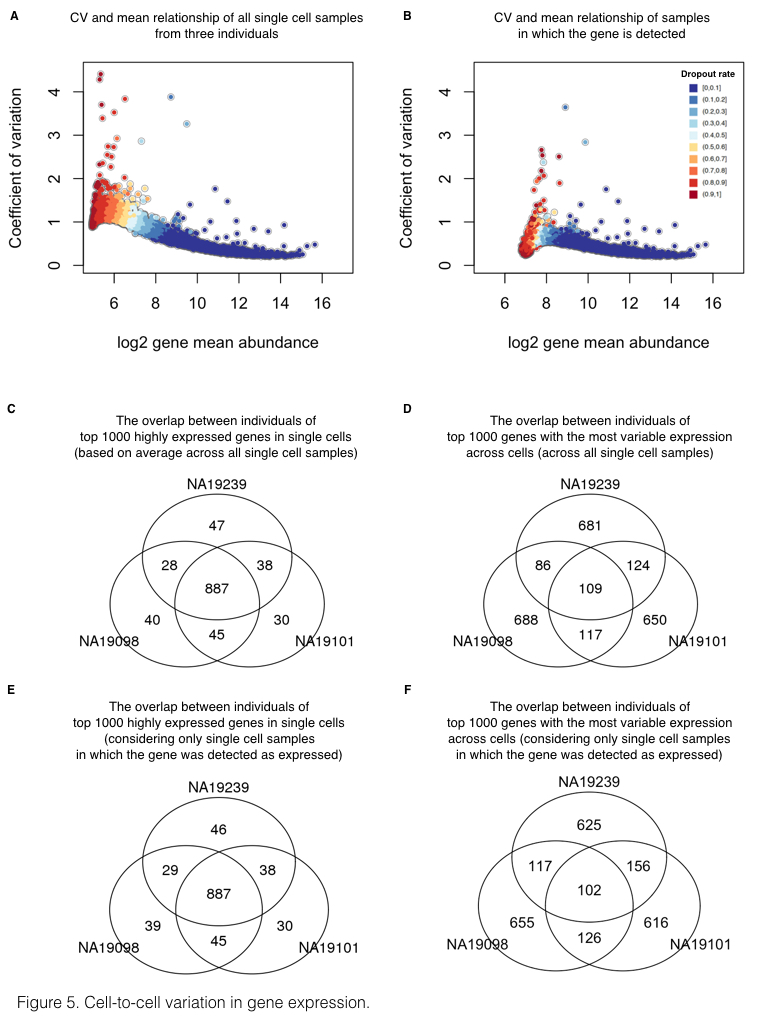
\includegraphics[trim=0 .5in 0 0,clip,width=5in]{img/ch04/Figure05.jpeg}
\caption{\textbf{Figure 5. Cell-to-cell variation in gene expression.}
Adjusted CV plotted against average molecule counts across all cells in
(A) and across only the cells in which the gene is expressed (B),
including data from all three individuals. Each dot represents a gene,
and the color indicates the corresponding gene-specific dropout rate
(the proportion of cells in which the gene is undetected). (C and D)
Venn diagrams showing the overlaps of top 1000 genes across individuals
based on mean expression level in (C) and based on adjusted CV values in
(D), considering only the cells in which the gene is expressed. (E and
F) Similarly, Venn diagrams showing the overlaps of top 1000 genes
across individuals based on mean expression level in (E) and based on
adjusted CV values in (F), across all cells.}
\end{figure}

\section{Discussion}\label{discussion}

\subsection{Study design and sample size for
scRNA-seq}\label{study-design-and-sample-size-for-scrna-seq}

Our nested study design allowed us to explicitly estimate technical
batch effects associated with single cell sample processing on the C1
platform. We found previously unreported technical sources of variation
associated with the C1 sample processing and the use of UMIs, including
the property of batch-specific read-to-molecule conversion efficiency.
As we used a well-replicated nested study design, we were able to model,
estimate, and account for the batch while maintaining individual
differences in gene expression levels. We believe that our observations
indicate that future studies should avoid confounding C1 batch and
individual source of single cell samples. Instead, we recommend a
balanced study design consisting of multiple individuals within a C1
plate and multiple C1 replicates (for example, Supplementary Fig. S8).
The origin of each cell can then be identified using the RNA sequencing
data. Indeed, using a method originally developed for detecting sample
swaps in DNA sequencing experiments \citep{Jun2012}, we were able to
correctly identify the correct YRI individual of origin for all the
single cells from the current experiment by comparing the polymorphisms
identified using the RNA-seq reads to the known genotypes for all 120
YRI individuals of the International HapMap Project
\citep{HapMapConsortium2005} (Supplementary Fig. S8). The
mixed-individual-plate is an attractive study design because it allows
one to account for the batch effect without the requirement to
explicitly spend additional resources on purely technical replication
(because the total number of cells assayed from each individual can be
equal to a design in which one individual is being processed in using a
single C1 plate).

We also addressed additional study design properties with respect to the
desired number of single cells and the desired depth of sequencing (Fig.
2). Similar assessments have been previously performed for single cell
sequencing with the C1 platform without the use of UMIs \citep{Wu2014,
Pollen2014}, but no previous study has investigated the effects of
these parameters for single cells studies using UMIs. We focused on
recapitulating the gene expression levels observed in bulk sequencing
experiments, detecting as many genes as possible, and accurately
measuring the cell-to-cell variation in gene expression levels. We
recommend sequencing at least 75 high quality cells per biological
condition with a minimum of 1.5 million raw reads per cell to obtain
optimal performance of these three metrics.

\subsection{The limitations of the ERCC spike-in
controls}\label{the-limitations-of-the-ercc-spike-in-controls}

The ERCC spike-in controls have been used in previous scRNA-seq studies
to identify low quality single cell samples, infer the absolute total
number of molecules per cell, and model the technical variability across
cells \citep{Brennecke2013, Grun2014, Ding2015, Vallejos2015}. In our
experience, the ERCC controls are not particularly well-suited for any
one of these tasks, much less all three. With respect to identifying low
quality samples, we indeed observed that samples with no visible cell
had a higher percentage of reads mapping to the ERCC controls, as
expected. However, there was no clear difference between low and high
quality samples in the percentage of ERCC reads or molecules, and thus
any arbitrarily chosen cutoff would be associated with considerable
error (Fig. 1E). With respect to inferring the absolute total number of
molecules per cell, we observed that the biological covariate of
interest (difference between the three YRI individuals), rather than
batch, explained a large proportion of the variance in the ERCC counts
(Supplementary Fig. S3), and furthermore that the ERCC controls were
also affected by the individual-specific effect on the read-to-molecule
conversion rate (Fig. 3D). Thus ERCC-based corrected estimates of total
number of molecules per cell, across technical or biological replicates,
are expected to be biased. Because the batch effects associated with the
ERCC controls are driven by the biological covariate of interest, they
will also impede the modeling of the technical variation in single cell
experiments that confound batch and the biological source of the single
cells.

More generally, it is inherently difficult to model unknown sources of
technical variation using so few genes \citep{Risso2014} (only
approximately half of the 92 ERCC controls are detected in typical
single cell experiments), and the ERCC controls are also strongly
impacted by technical sources of variation even in bulk RNA-seq
experiments \citep{SEQC/MAQC-IIIConsortium2014}. Lastly, from a
theoretical perspective, the ERCC controls have shorter polyA tails and
are overall shorter than mammalian mRNAs. For these reasons, we caution
against the reliance of ERCC controls in scRNA-seq studies and highlight
that an alternative set of controls that more faithfully mimics
mammalian mRNAs and provides more detectable spike-in genes is desired.
Our recommendation is to include total RNA from a distant species, for
example using RNA from \emph{Drosophila} \emph{melanogaster} in studies
of single cells from humans.

\subsection{Outlook}\label{outlook}

Single cell experiments are ideally suited to study gene regulatory
noise and robustness \citep{Borel2015, Finak2015}. Yet, in order to
study the biological noise in gene expression levels, it is imperative
that one should be able to effectively estimate and account for the
technical noise in single cell gene expression data. Our results
indicate that previous single cells gene expression studies may not have
been able to distinguish between the technical and the biological
components of variation, because single cell samples from each
biological condition were processed on a single C1 batch. When technical
noise is properly accounted for, even in this small pilot study, our
findings indicate pervasive inter-individual differences in gene
regulatory noise, independently of the overall gene expression level.

\section{Methods}\label{methods}

\subsection{Ethics statement}\label{ethics-statement}

The YRI cell lines were purchased from CCR. The original samples were
collected by the HapMap project between 2001-2005. All of the samples
were collected with extensive community engagement, including
discussions with members of the donor communities about the ethical and
social implications of human genetic variation research. Donors gave
broad consent to future uses of the samples, including their use for
extensive genotyping and sequencing, gene expression and proteomics
studies, and all other types of genetic variation research, with the
data publicly released.

\subsection{Cell culture of iPSCs}\label{cell-culture-of-ipscs}

Undifferentiated feeder-free iPSCs reprogrammed from LCLs of Yoruba
individuals in Ibadan, Nigeria (abbreviation: YRI)
\citep{HapMapConsortium2005} were grown in E8 medium (Life Technologies)
\citep{Chen2011} on Matrigel-coated tissue culture plates with daily
media feeding at 37 °C with 5\% (vol/vol) CO2. For standard maintenance,
cells were split every 3-4 days using cell release solution (0.5 mM EDTA
and NaCl in PBS) at the confluence of roughly 80\%. For the single cell
suspension, iPSCs were individualized by Accutase Cell Detachment
Solution (BD) for 5-7 minutes at 37 °C and washed twice with E8 media
immediately before each experiment. Cell viability and cell counts were
then measured by the Automated Cell Counter (Bio-Rad) to generate
resuspension densities of 2.5 X 105 cells/mL in E8 medium for C1 cell
capture.

\subsection{Single cell capture and library
preparation}\label{single-cell-capture-and-library-preparation}

Single cell loading and capture were performed following the Fluidigm
protocol (PN 100-7168). Briefly, 30 $\mu$l of C1 Suspension Reagent was
added to a 70-$\mu$l aliquot of \textasciitilde{}17,500 cells. Five
$\mu$l of this cell mix were loaded onto 10-17 $\mu$m C1 Single-Cell
Auto Prep IFC microfluidic chip (Fluidigm), and the chip was then
processed on a C1 instrument using the cell-loading script according to
the manufacturer's instructions. Using the standard staining script, the
iPSCs were stained with StainAlive TRA-1-60 Antibody (Stemgent, PN
09-0068). The capture efficiency and TRA-1-60 staining were then
inspected using the EVOS FL Cell Imaging System (Thermo Fisher)
(Supplementary Table S1).

Immediately after imaging, reverse transcription and cDNA amplification
were performed in the C1 system using the SMARTer PCR cDNA Synthesis kit
(Clontech) and the Advantage 2 PCR kit (Clontech) according to the
instructions in the Fluidigm user manual with minor changes to
incorporate UMI labeling \citep{Islam2014}. Specifically, the reverse
transcription primer and the 1:50,000 Ambion® ERCC Spike-In Mix1 (Life
Technologies) were added to the lysis buffer, and the template-switching
RNA oligos which contain the UMI (5-bp random sequence) were included in
the reverse transcription mix \citep{Islam2011, Islam2012, Islam2014}.
When the run finished, full-length, amplified, single-cell cDNA
libraries were harvested in a total of approximately 13 $\mu$l C1
Harvesting Reagent and quantified using the DNA High Sensitivity LabChip
(Caliper). The average yield of samples per C1 plate ranged from
1.26-1.88 ng per microliter (Supplementary Table S1). A bulk sample, a
40 $\mu$l aliquot of \textasciitilde{}10,000 cells, was collected in
parallel with each C1 chip using the same reaction mixes following the
C1 protocol (PN 100-7168, Appendix A).

For sequencing library preparation, tagmentation and isolation of 5'
fragments were performed according to the UMI protocol \citep{Islam2014}.
Instead of using commercially available Tn5 transposase, Tn5 protein
stock was freshly purified in house using the IMPACT system (pTXB1, NEB)
following the protocol previously described \citep{Picelli2014}. The
activity of Tn5 was tested and shown to be comparable with the
EZ-Tn5-Transposase (Epicentre). Importantly, all the libraries in this
study were generated using the same batch of Tn5 protein purification.
For each of the bulk samples, two libraries were generated using two
different indices in order to get sufficient material for sequencing.
All 18 bulk libraries were then pooled and labeled as the ``bulk'' for
sequencing.

\subsection{Illumina high-throughput
sequencing}\label{illumina-high-throughput-sequencing}

The scRNA-seq libraries generated from the 96 single cell samples of
each C1 chip were pooled and then sequenced in three lanes on an
Illumina HiSeq 2500 instrument using the PCR primer (C1-P1-PCR-2:
Bio-GAATGATACGGCGACCACCGAT) as the read 1 primer and the Tn5 adapter
(C1-Tn5-U: PHO-CTGTCTCTTATACACATCTGACGC) as the index read primer
following the UMI protocol \citep{Islam2014}.

The master mixes, one mix with all the bulk samples and nine mixes
corresponding to the three replicates for the three individuals, were
sequenced across four flowcells using a design aimed to minimize the
introduction of technical batch effects (Supplementary Table S1).
Single-end 100 bp reads were generated along with 8-bp index reads
corresponding to the cell-specific barcodes. We did not observe any
obvious technical effects due to sequencing lane or flow cell that
confounded the inter-individual and inter-replicate comparisons.

\subsection{Read mapping}\label{read-mapping}

To assess read quality, we ran FastQC
(\url{http://www.bioinformatics.babraham.ac.uk/projects/fastqc}) and
observed a decrease in base quality at the 3' end of the reads. Thus we
removed low quality bases from the 3' end using sickle with default
settings \citep{Joshi2011}. To handle the UMI sequences at the 5' end of
each read, we used umitools \citep{umitools} to find all reads with a UMI
of the pattern NNNNNGGG (reads without UMIs were discarded). We then
mapped reads to human genome hg19 (only including chromosomes 1-22, X,
and Y, plus the ERCC sequences) with Subjunc \citep{Liao2013}, discarding
non-uniquely mapped reads (option -u). To obtain gene-level counts, we
assigned reads to protein-coding genes (Ensembl GRCh37 release 82) and
the ERCC spike-in genes using featureCounts \citep{Liao2014}. Because the
UMI protocol maintains strand information, we required that reads map to
a gene in the correct orientation (featureCounts flag -s 1).

In addition to read counts, we utilized the UMI information to obtain
molecule counts for the single cell samples. We did not count molecules
for the bulk samples because this would violate the assumptions of the
UMI protocol, as bulk samples contain far too many unique molecules for
the 1,024 UMIs to properly tag them all. First, we combined all reads
for a given single cell using samtools \citep{Li2009}. Next, we converted
read counts to molecule counts using UMI-tools \citep{Smith2016}.
UMI-tools counts the number of UMIs at each read start position.
Furthermore, it accounts for sequencing errors in the UMIs introduced
during the PCR amplification or sequencing steps using a ``directional
adjacency'' method. Briefly, all UMIs at a given read start position are
connected in a network using an edit distance of one base pair. However,
edges between nodes (the UMIs) are only formed if the nodes have less
than a 2x difference in reads. The node with the highest number of reads
is counted as a unique molecule, and then it and all connected nodes are
removed from the network. This is repeated until all nodes have been
counted or removed.

\subsection{Filtering cells and
genes}\label{filtering-cells-and-genes}

We performed multiple quality control analyses to detect and remove data
from low quality cells. In an initial analysis investigating the
percentage of reads mapping to the ERCC spike-in controls, we observed
that replicate 2 of individual NA19098 was a clear outlier
(Supplementary Fig. S1). It appeared that too much ERCC spike-in mix was
added to this batch, which violated the assumption that the same amount
of ERCC molecules was added to each cell. Thus, we removed this batch
from all of our analyses.

Next, we kept data from high quality single cells that passed the
following criteria:

\begin{itemize}
\itemsep1pt\parskip0pt\parsep0pt
\item
  Only one cell observed per well
\item
  At least 1,556,255 mapped reads
\item
  Less than 36.4\% unmapped reads
\item
  Less than 3.2\% ERCC reads
\item
  More than 6,788 genes with at least one read
\end{itemize}

We chose the above criteria based on the distribution of these metrics
in the empty wells (the cutoff is the 95th percentile, Supplementary
Fig. S1). In addition, we observed that some wells classified as
containing only one cell were clustered with multi-cell wells when
plotting 1) the number of gene molecules versus the concentration of the
samples, and 2) the read to molecule conversion efficiency (total
molecule number divided by total read number) of endogenous genes versus
that of ERCC. We therefore established filtering criteria for these
misidentified single-cell wells using linear discriminant analysis
(LDA). Specifically, LDA was performed to classify wells into empty,
one-cell, and two-cell using the discriminant functions of 1) sample
concentration and the number of gene molecules, and 2) endogenous and
ERCC gene read to molecule conversion efficiency (Supplementary Fig.
S2). After filtering, we maintained 564 high quality single cells
(NA19098: 142, NA19101: 201, NA19239: 221).

The quality control analyses were performed using all protein-coding
genes (Ensembl GRCh37 release 82) with at least one observed read. Using
the high quality single cells, we further removed genes with low
expression levels for downstream analyses. We removed all genes with a
mean log\textsubscript{2} cpm less than 2, which did not affect the
relative differences in the proportion of genes detected across batches
(Supplementary Fig. S9). We also removed genes with molecule counts
larger than 1,024 for the correction of collision probability. In the
end we kept 13,058 endogenous genes and 48 ERCC spike-in genes.

\subsection{Calculate the input molecule quantities of ERCC
spiked-ins}\label{calculate-the-input-molecule-quantities-of-ercc-spiked-ins}

According to the information provided by Fluidigm, each of the 96
capture chamber received 13.5 nl of lysis buffer, which contain 1:50,000
Ambion® ERCC Spike-In Mix1 (Life Technologies) in our setup. Therefore,
our estimation of the total spiked-in molecule number was 16,831 per
sample. Since the relative concentrations of the ERCC genes were
provided by the manufacturer, we were able to calculate the molecule
number of each ERCC gene added to each sample. We observed that the
levels of ERCC spike-ins strongly correlated with the input quantities
(r = 0.9914, Fig. 1G). The capture efficiency, defined as the fraction
of total input molecules being successfully detected in each high
quality cell, had an average of 6.1\%.

\subsection{Subsampling}\label{subsampling}

We simulated different sequencing depths by randomly subsampling reads
and processing the subsampled data through the same pipeline described
above to obtain the number of molecules per gene for each single cell.
To assess the impact of sequencing depth and number of single cells, we
calculated the following three statistics:

\begin{enumerate}
\def\labelenumi{\arabic{enumi}.}
\itemsep1pt\parskip0pt\parsep0pt
\item
  The Pearson correlation of the gene expression level estimates from
  the single cells compared to the bulk samples. For the single cells,
  we summed the gene counts across all the samples and then calculated
  the log\textsubscript{2} cpm of this pseudo-bulk. For the bulk
  samples, we calculated the log\textsubscript{2} cpm separately for
  each of the three replicates and then calculated the mean per gene.
\item
  The number of genes detected with at least one molecule in at least
  one cell.
\item
  The Pearson correlation of the cell-to-cell gene expression variance
  estimates from the subsampled single cells compared to the variance
  estimates using the full single cell data set.
\end{enumerate}

Each data point in Fig. 2 represents the mean +/- the standard error of
the mean (SEM) of 10 random subsamples of cells. We split the genes by
expression level into two groups (6,097 genes each) to highlight that
most of the improvement with increased sequencing depth and number of
cells was driven by the estimates of the lower half of expressed genes.
The data shown is for individual NA19239, but the results were
consistent for individuals NA19098 and NA19101. Only high quality single
cells (Supplementary Table S2) were included in this analysis.

\subsection{A framework for testing individual and batch
effects}\label{a-framework-for-testing-individual-and-batch-effects}

Individual effect and batch effect between the single cell samples were
evaluated in a series of analyses that examine the potential sources of
technical variation on gene expression measurements. These analyses took
into consideration that in our study design, sources of variation
between single cell samples naturally fall into a hierarchy of
individuals and C1 batches. In these sample-level analyses, the
variation introduced at both the individual-level and the batch-level
was modeled in a nested framework that allows random noise between C1
batches within individuals. Specifically, for each cell sample in
individual $i$, replicate $j$ and well $k$, we used $y_{ijk}$ to denote
some sample measurement (e.g.~total molecule-counts) and fit a linear
mixed model with the fixed effect of individual $\alpha_i$ and the
random effect of batch $b_{ij}$:

\[y_{ijk} = \alpha_{i} + b_{ij} + \epsilon_{ijk} \,\,\,\,(1)\]

where the random effect $b_{ij}$ of batch follows a normal distribution
with mean zero and variance $\sigma^2_{b}$, and $\epsilon_{ijk}$
describes residual variation in the sample measurement. To test the
statistical significance of individual effect (i.e., null hypothesis
$\alpha_1 = \alpha_2 = \alpha_3$), we performed a likelihood ratio test
(LRT) to compare the above full model and the reduced model that
excludes $\alpha_i$. To test if there was a batch effect (i.e., null
hypothesis $\sigma^2_b = 0$), we performed an F-test to compare the
variance that is explained by the above full model and the variance due
to the reduced model that excludes $b_{ij}$.

The nested framework was applied to test the individual and batch
effects between samples in the following cases. The data includes
samples after quality control and filtering.

\begin{enumerate}
\def\labelenumi{\arabic{enumi}.}
\item
  Total molecule count (on the log\textsubscript{2} scale) was modeled
  as a function of individual effect and batch effect, separately for
  the ERCC spike-ins and for the endogenous genes.
\item
  Read-to-molecule conversion efficiency was modeled as a function of
  individual effect and batch effect, separately for the ERCC spike-ins
  and for the endogenous genes.
\end{enumerate}

\subsection{Estimating variance components for per-gene expression
levels}\label{estimating-variance-components-for-per-gene-expression-levels}

To assess the relative contributions of individual and technical
variation, we analyzed per-gene expression profiles and computed
variance component estimates for the effects of individual and C1 batch
(Supplementary Fig. S3). The goal here was to quantify the proportion of
cell-to-cell variance due to individual (biological) effect and to C1
batch (technical) at the per-gene level. Note that the goal here was
different from that of the previous section, where we simply tested for
the existence of individual and batch effects at the sample level by
rejecting the null hypothesis of no such effects. In contrast, here we
fit a linear mixed model per gene where the dependent variable was the
gene expression level (log\textsubscript{2} counts per million) and the
independent variables were individual and batch, both modeled as random
effects.

The variance parameters of individual effect and batch effect were
estimated using a maximum penalized likelihood approach
\citep{Chung2013}, which can effectively avoid the common issue of zero
variance estimates due to small sample sizes (there were three
individuals and eight batches). We used the blmer function in the R
package blme and set the penalty function to be the logarithm of a gamma
density with shape parameter = 2 and rate parameter tending to zero.

The estimated variance components were used to compute the sum of
squared deviations for individual and batch effects. The proportion of
variance due to each effect is equal to the relative contribution of the
sum of squared deviations for each effect compared to the total sum of
squared deviations per gene. Finally, we compared the estimated
proportions of variance due to the individual effect and the batch
effect, across genes, using a non-parametric one-way analysis of
variance (Kruskal-Wallis rank sum test).

\subsection{Normalization}\label{normalization}

We transformed the single cell molecule counts in multiple steps (Fig.
4). First, we corrected for the collision probability using a method
similar to that developed by Grün et al. \citep{Grun2014}. Essentially we
corrected for the fact that we did not observe all the molecules
originally in the cell. The main difference between our approach and
that of Grün et al. \citep{Grun2014} was that we applied the correction
at the level of gene counts and not individual molecule counts. Second,
we standardized the molecule counts to log\textsubscript{2} counts per
million (cpm). This standardization was performed using only the
endogenous gene molecules and not the ERCC molecules. Third, we
corrected for cell-to-cell technical noise using the ERCC spike-in
controls. For each single cell, we fit a Poisson generalized linear
model (GLM) with the log\textsubscript{2} expected ERCC molecule counts
as the independent variable, and the observed ERCC molecule counts as
the dependent variable, using the standard log link function. Next we
used the slope and intercept of the Poisson GLM regression line to
transform the log\textsubscript{2} cpm for the endogenous genes in that
cell. This is analogous to the standard curves used for qPCR
measurements, but taking into account that lower concentration ERCC
genes will have higher variance from Poisson sampling. Fourth, we
removed technical noise between the eight batches (three replicates each
for NA19101 and NA19239 and two replicates for NA19098). We fit a linear
mixed model with a fixed effect for individual and a random effect for
the eight batches and removed the variation captured by the random
effect (see the next section for a detailed explanation).

For the bulk samples, we used read counts even though the reads
contained UMIs. Because these samples contained RNA molecules from
\textasciitilde{}10,000 cells, we could not assume that the 1,024 UMIs
were sufficient for tagging such a large number of molecules. We
standardized the read counts to log\textsubscript{2} cpm.

\subsection{Removal of technical batch
effects}\label{removal-of-technical-batch-effects}

Our last normalization step adjusted the transformed
log\textsubscript{2} gene expression levels for cell-to-cell correlation
within each C1 plate. The algorithm mimics a method that was initially
developed for adjusting within-replicate correlation in microarray data
\citep{Smyth2005}. We assumed that for each gene $g$, cells that belong
to the same batch $j$ are correlated, for batches $j = 1, \dots, 8$. The
batch effect is specific to each C1 plate and is independent of
biological variation across individuals.

We fit a linear mixed model for each gene $g$ that includes a fixed
effect of individual and a random effect for within-batch variation
attributed to cell-to-cell correlation in each C1 plate:

\[ y_{g,ijk} = \mu_{g} + \alpha_{g,i} + b_{g,ij} + \epsilon_{g,ijk}, \,\,\,\,(2)\]

where $y_{g,ijk}$ denotes log\textsubscript{2} counts-per-million (cpm)
of gene $g$ in individual $i$, replicate $j$, and cell $k$;
$i = NA19098, NA19101, NA19239$, $j = 1, \dots, n_i$ with $n_i$ the
number of replicates in individual $i$, $k = 1, \dots, n_{ij}$ with
$n_{ij}$ the number of cells in individual $i$ replicate $j$. $\mu_g$
denotes the mean gene expression level across cells, $\alpha_{g,i}$
quantifies the individual effect on mean gene expression, $b_{g,ij}$
models the replicate effect on mean expression level (assumed to be
stochastic, independent, and identically distributed with mean 0 and
variance $\sigma^2_{g,b}$). Finally, $\epsilon_{g,ijk}$ describes the
residual variation in gene expression.

Batch-corrected expression levels were computed as

\[ \widehat{y}_{g,ijk} = y_{g,ijk} - \widehat{b}_{g,ij}, \,\,\,\,(3)\]

where $\widehat{b}_{g,ij}$ are the least-squares estimates. The
computations in this step were done with the gls.series function of the
limma package \citep{limma}.

\subsection{Measurement of gene expression
noise}\label{measurement-of-gene-expression-noise}

While examining gene expression noise (using the coefficient of
variation or CV) as a function of mean RNA abundance across C1
replicates, we found that the CV of molecule counts among endogenous
genes and ERCC spike-in controls suggested similar expression
variability patterns. Both endogenous and ERCC spike-in control CV
patterns approximately followed an over-dispersed Poisson distribution
(Supplementary Fig. S10), which is consistent with previous studies
\citep{Islam2014, Brennecke2013}. We computed a measure of gene
expression noise that is independent of RNA abundance across individuals
\citep{Kolodziejczyk2015, Newman2006}. First, squared coefficients of
variation (CVs) for each gene were computed for each individual and also
across individuals, using the batch-corrected molecule data. Then we
computed the distance of individual-specific CVs to the rolling median
of global CVs among genes that have similar RNA abundance levels. These
transformed individual CV values were used as our measure of gene
expression noise. Specifically, we computed the adjusted CV values as
follows:

\begin{enumerate}
\def\labelenumi{\arabic{enumi}.}
\item
  Compute squared CVs of molecule counts in each individual and across
  individuals.
\item
  Order genes by the global average molecule counts.
\item
  Starting from the genes with the lowest global average gene expression
  level, for every sliding window of 50 genes, subtract
  log\textsubscript{10} median squared CVs from log\textsubscript{10}
  squared CVs of each cell line, and set 25 overlapping genes between
  windows. The computation was performed with the rollapply function of
  the R zoo package \citep{Zeileis2005}. After this transformation step,
  CV no longer had a polynomial relationship with mean gene molecule
  count (Supplementary Fig. S10).
\end{enumerate}

\subsection{Identification of genes associated with inter-individual
differences in regulatory
noise}\label{identification-of-genes-associated-with-inter-individual-differences-in-regulatory-noise}

To identify differential noise genes across individuals, we computed
median absolute deviation (MAD) - a robust and distribution-free
dissimilarity measure for gene $g$:

\[ MAD_{g} = Median_{i= 1,2,3} \left| \text{adjCV}_{g,i} -  Median_{i= 1,2,3} ({\text{adjCV}}_{g,i}) \right|. \,\,\,\,(4)\]

Large values of $MAD_{g}$ suggest a large deviation from the median of
the adjusted CV values. We identified genes with significant
inter-individual differences using a permutation-based approach.
Specifically, for each gene, we computed empirical \emph{P}-values based
on 300,000 permutations. In each permutation, the sample of origin
labels were shuffled between cells. Because the number of permutations
in our analysis was smaller than the maximum possible number of
permutations, we computed the empirical \emph{P}-values as
$\frac{b + 1}{m + 1}$, where \emph{b} is the number of permuted MAD
values greater than the observed MAD value, and \emph{m} is the number
of permutations. Adding 1 to \emph{b} avoided an empirical
\emph{P}-value of zero \citep{Phipson2010}.

\subsection{Gene enrichment analysis}\label{gene-enrichment-analysis}

We used ConsensusPATHDB \citep{Kamburov2011} to identify GO terms that
are over-represented for genes whose variation in single cell expression
levels were significantly difference between individuals.

\subsection{Individual assignment based on scRNA-seq
reads}\label{individual-assignment-based-on-scrna-seq-reads}

We were able to successfully determine the correct identity of each
single cell sample by examining the SNPs present in their RNA sequencing
reads. Specifically, we used the method verifyBamID
(\url{https://github.com/statgen/verifyBamID}) developed by Jun et al.,
2012 \citep{Jun2012}, which detects sample contamination and/or
mislabeling by comparing the polymorphisms observed in the sequencing
reads for a sample to the genotypes of all individuals in a study. For
our test, we included the genotypes for all 120 Yoruba individuals that
are included in the International HapMap Project
\citep{HapMapConsortium2005}. The genotypes included the HapMap SNPs with
the 1000 Genomes Project SNPs \citep{OneKGConsortium2012} imputed, as
previously described \citep{McVicker2013}. We subset to include only the
528,289 SNPs that overlap Ensembl protein-coding genes. verifyBamID used
only 311,848 SNPs which passed its default thresholds (greater than 1\%
minor allele frequency and greater than 50\% call rate). Using the
option --best to return the best matching individual, we obtained 100\%
accuracy identifying the single cells of all three individuals
(Supplementary Fig. S8).

\subsection{Data and code
availability}\label{data-and-code-availability}

The data have been deposited in NCBI's Gene Expression Omnibus
\citep{Edgar2002} and are accessible through GEO Series accession number
GSE77288
(\url{http://www.ncbi.nlm.nih.gov/geo/query/acc.cgi?acc=GSE77288}). The
code and processed data are available at
\url{https://github.com/jdblischak/singleCellSeq}. The results of our
analyses are viewable at
\url{https://jdblischak.github.io/singleCellSeq/analysis}.

\section{Acknowledgments}\label{acknowledgments}

We thank members of the Pritchard, Gilad, and Stephens laboratories for
valuable discussions during the preparation of this manuscript. This
work was funded by NIH grant HL092206 to YG and HHMI funds to JKP. PYT
is supported by NIH T32HL007381. JDB was supported by NIH T32GM007197.
The content is solely the responsibility of the authors and does not
necessarily represent the official views of the National Institutes of
Health.

\section{Author Contributions}\label{author-contributions}

YG and JKP conceived of the study, designed the experiments, and
supervised the project. PT and JEB performed the experiments. PT, JDB,
CH, and DAK analyzed the results. PT, JDB, CH, and YG wrote the original
draft. All authors reviewed the final manuscript.

\section{Competing financial
interests}\label{competing-financial-interests}

The authors declare no competing financial interests.

\clearpage
\section{Supplementary Information}\label{supplementary-information}

\subsection{Supplementary Figures}\label{supplementary-figures}

\begin{figure}[htbp]
\centering
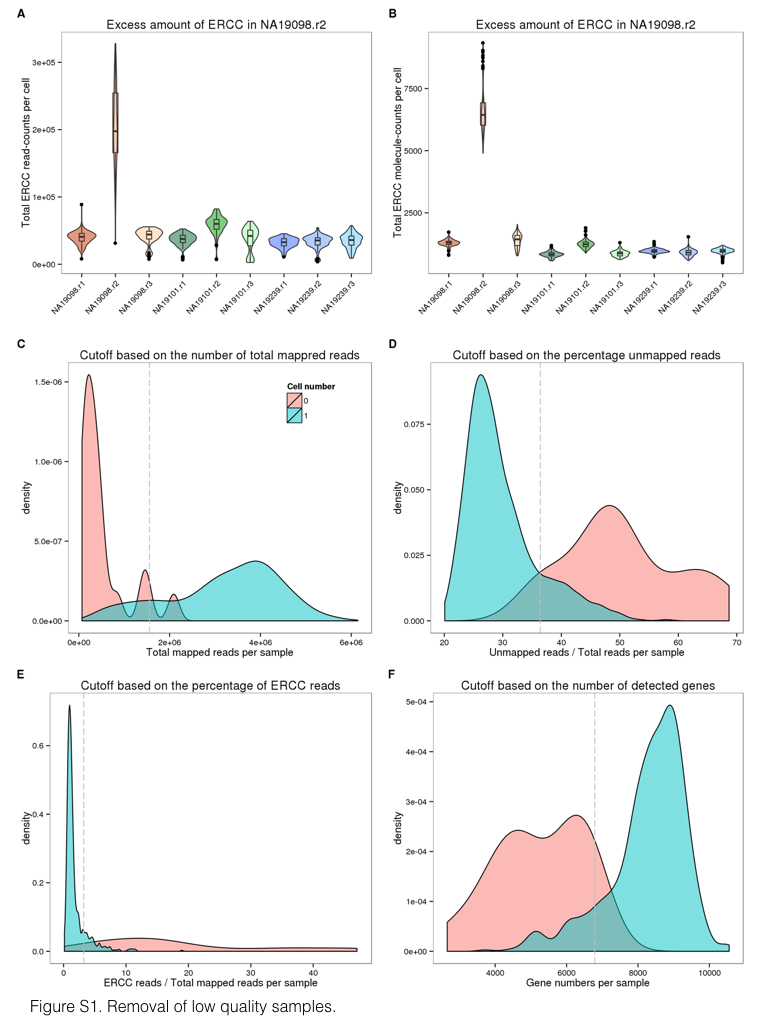
\includegraphics[trim=0 .5in 0 0,clip,width=5in]{img/ch04/Figure06.jpeg}
\caption{\textbf{Supplementary Figure S1. Removal of low quality
samples.} Violin plots of the total read-counts of ERCC spike-in
controls in (A) and the total molecule-counts in (B) in single cell
samples. The three colors represent the three individuals (NA19098 in
red, NA19101 in green, and NA19239 in blue). (C-F) Density plots of the
distributions of the total mapped reads in (C), the percentage of
unmapped reads in (D), the percentage of ERCC reads in (E), and the
number of detected genes in (F). The dash lines indicate the cutoffs
based on the 95th percentile of the samples with no cells.}
\end{figure}

\begin{figure}[htbp]
\centering
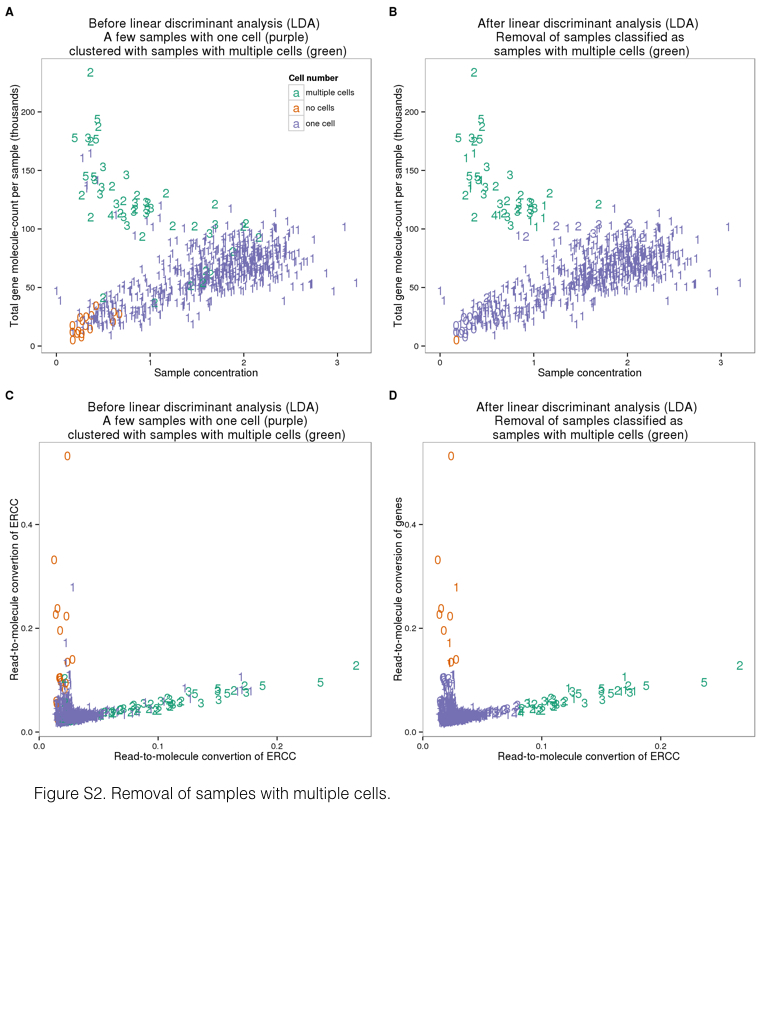
\includegraphics[trim=0 3.5in 0 0,clip,width=5in]{img/ch04/Figure07.jpeg}
\caption{\textbf{Supplementary Figure S2. Removal of samples with
multiple cells.} Scatterplots of the three groups of samples (no cell in
green, single-cell in orange, and two or more cells in purple) before
(A) and after (B) the linear discriminant analysis (LDA) using sample
concentration of cDNA amplicons (ng/$\mu$l) and the number of detected
genes. (C and D) Similarly, LDA was performed to identify potential
multi-cell samples using the read-to-molecule conversion efficiency
(total molecule-counts divided by total read-counts per sample) of
endogenous genes and ERCC spike-in controls. Scatterplots of before and
after the LDA in (C) and (D), respectively. The numbers indicate the
number of cells observed in each cell capture site.}
\end{figure}

\begin{figure}[htbp]
\centering
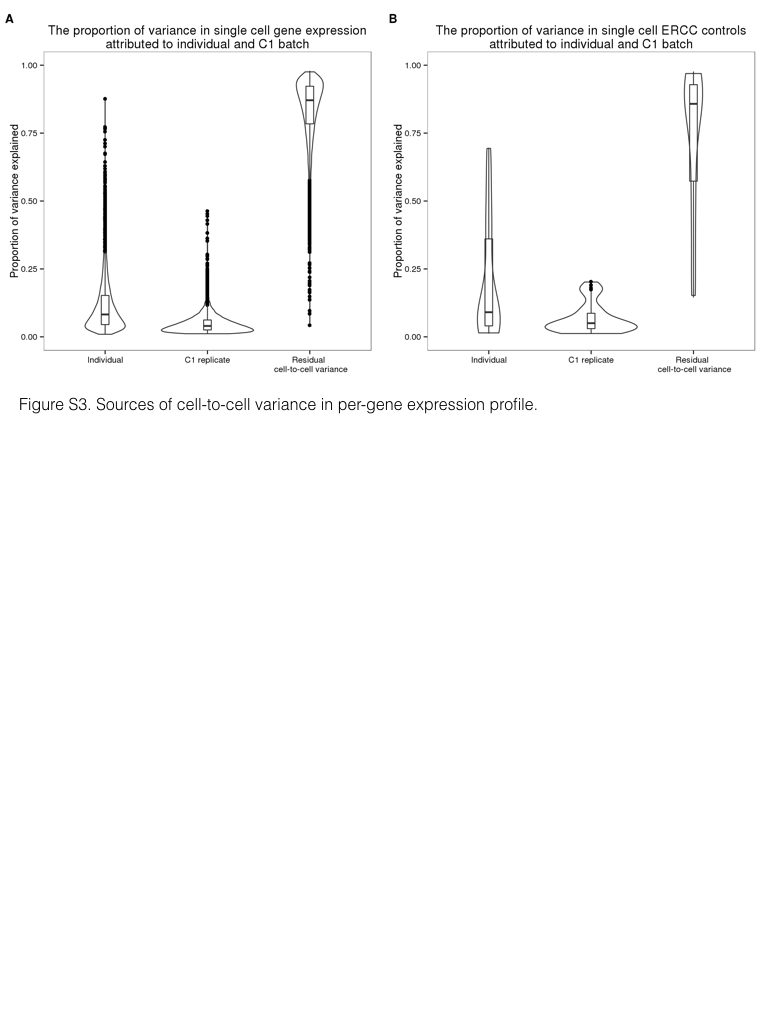
\includegraphics[trim=0 9in 0 0,clip,width=5in]{img/ch04/Figure08.jpeg}
\caption{\textbf{Supplementary Figure S3. Sources of cell-to-cell
variance in per-gene expression profile.} Violin plots of the proportion
of per-gene cell-to-cell variance that was due to individual sample of
origin, different C1 replicates, and other single cell sample
differences. These results were calculated from the molecule counts
before normalization and batch correction. Endogenous genes are shown in
(A) and the ERCC spike-in controls in (B).}
\end{figure}

\begin{figure}[htbp]
\centering
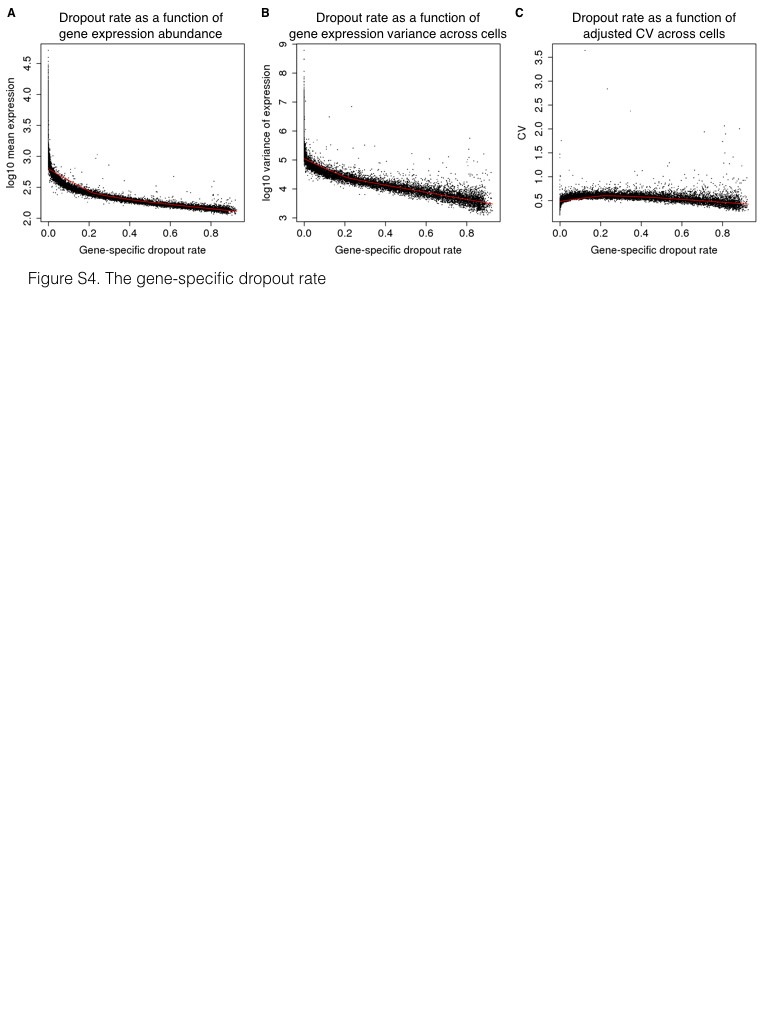
\includegraphics[trim=0 10.5in 0 0,clip,width=5in]{img/ch04/Figure09.jpeg}
\caption{\textbf{Supplementary Figure S4. The gene-specific dropout
rate.} The gene-specific dropout rate (the proportion of cells in which
the gene is undetected) and its relationship with log\textsubscript{10}
mean expression in (A), with log\textsubscript{10} variance of
expression in (B), and with the CV in (C) of the cells in which the gene
is expressed (cells in which at least one molecule of the given gene was
detected). Each point represents a gene, and red lines indicate the
predicted values using locally weighted scatterplot smoothing (LOESS).}
\end{figure}

\begin{figure}[htbp]
\centering
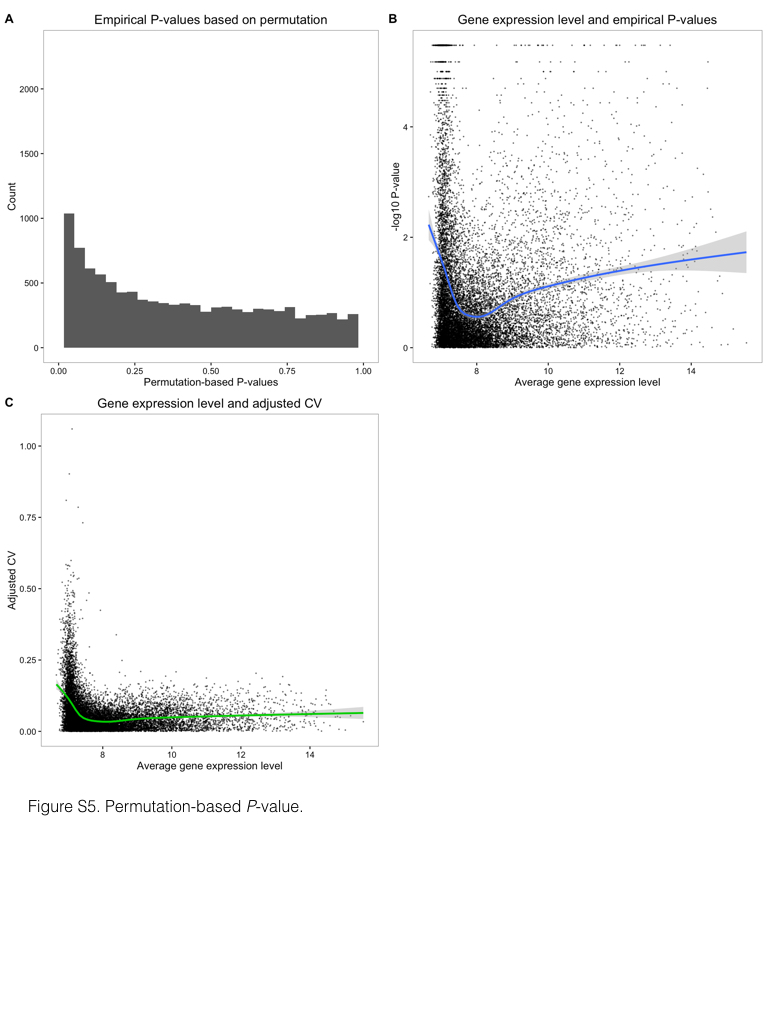
\includegraphics[trim=0 3.5in 0 0,clip,width=5in]{img/ch04/Figure10.jpeg}
\caption{\textbf{Supplementary Figure S5. Permutation-based
\emph{P}-value.} (A) Histogram of empirical \emph{P}-values based on
300,000 permutations. (B) -log\textsubscript{10} empirical
\emph{P}-values are plotted against average gene expression levels. Blue
line indicates the fitted relationship between -log\textsubscript{10}
\emph{P}-values and average log\textsubscript{2} gene expression levels
of cells that were detected as expressed, using locally weighted
scatterplot smoothing (LOESS). (C) Median of Absolute Deviation (MAD) of
genes versus average gene expression levels. Green line indicates the
fitted relationship (LOESS) between the MAD values and average
log\textsubscript{2} gene expression levels of cells in which the gene
was detected as expressed.}
\end{figure}

\begin{figure}[htbp]
\centering
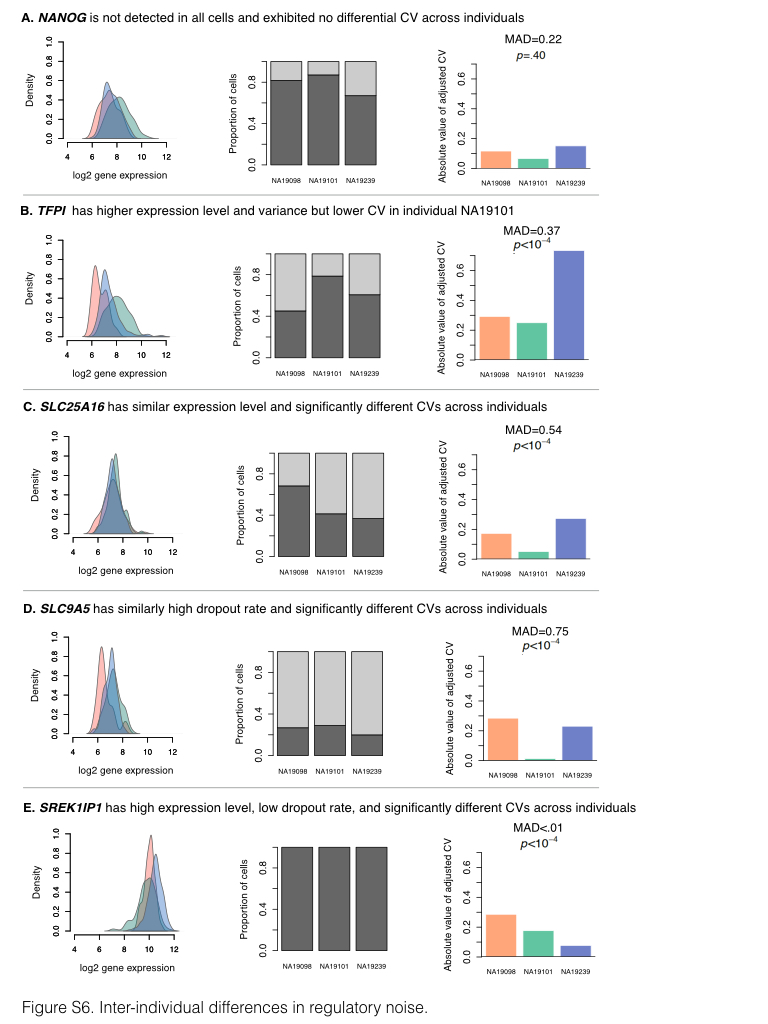
\includegraphics[trim=0 .5in 0 0,clip,width=5in]{img/ch04/Figure11.jpeg}
\caption{\textbf{Supplementary Figure S6. Inter-individual differences
in regulatory noise.} These 5 example genes illustrate various patterns
of cell-to-cell gene expression variance. For each gene, the left panel
shows the distribution of the log\textsubscript{2} gene expression
levels (considering only cells in which the gene is detected as
expressed), the middle panel shows the proportion of cells in which the
gene is detected as expressed (dark grey) and the dropout rate (light
grey) for each individual, and the right panel shows the absolute value
of adjusted CV for each individual, along with the corresponding
gene-specific MAD (median of absolute deviation) value and
\emph{P}-value. The three colors in the upper and lower panel represent
the individuals (NA19098 in red, NA19101 in green, and NA19239 in
blue).}
\end{figure}

\begin{figure}[htbp]
\centering
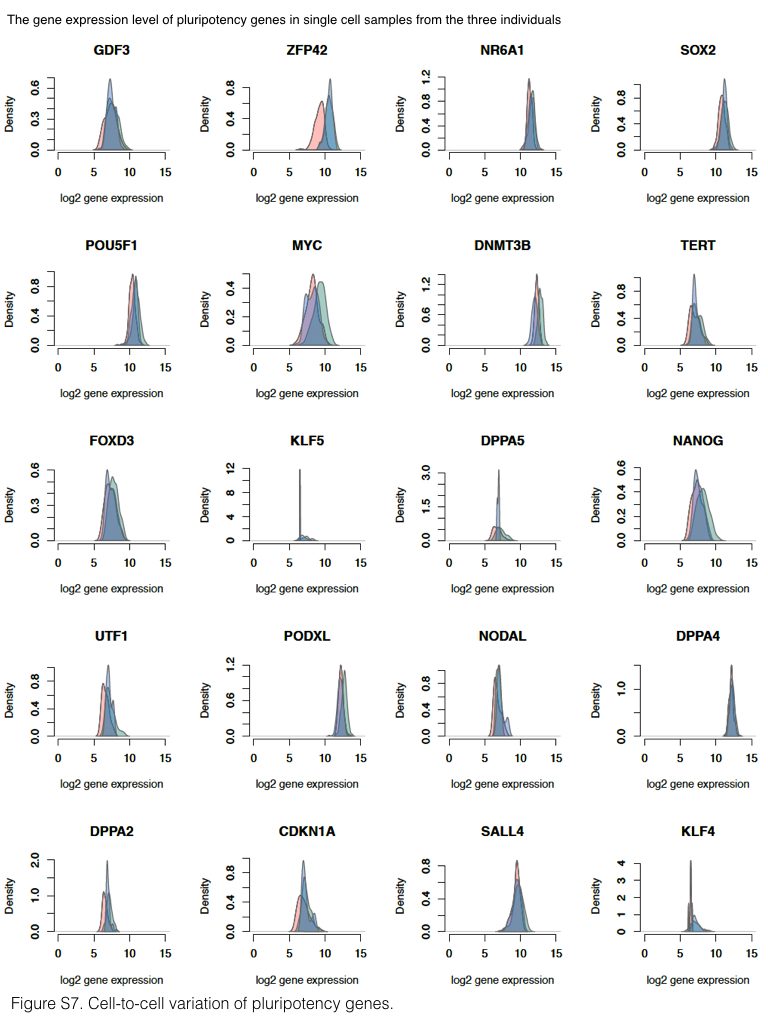
\includegraphics[trim=0 .5in 0 0,clip,width=5in]{img/ch04/Figure12.jpeg}
\caption{\textbf{Supplementary Figure S7. Cell-to-cell variation of
pluripotency genes.} Density plots of the distribution of
log\textsubscript{2} gene expression of key pluripotency genes across
all single cells by individual. The peaks with lower gene expression
values (log2 around 4) represent the cells in which the gene is
undetected. The three colors represent the three individuals (NA19098 is
in red, NA19101 in green, and NA19239 in blue).}
\end{figure}

\begin{figure}[htbp]
\centering
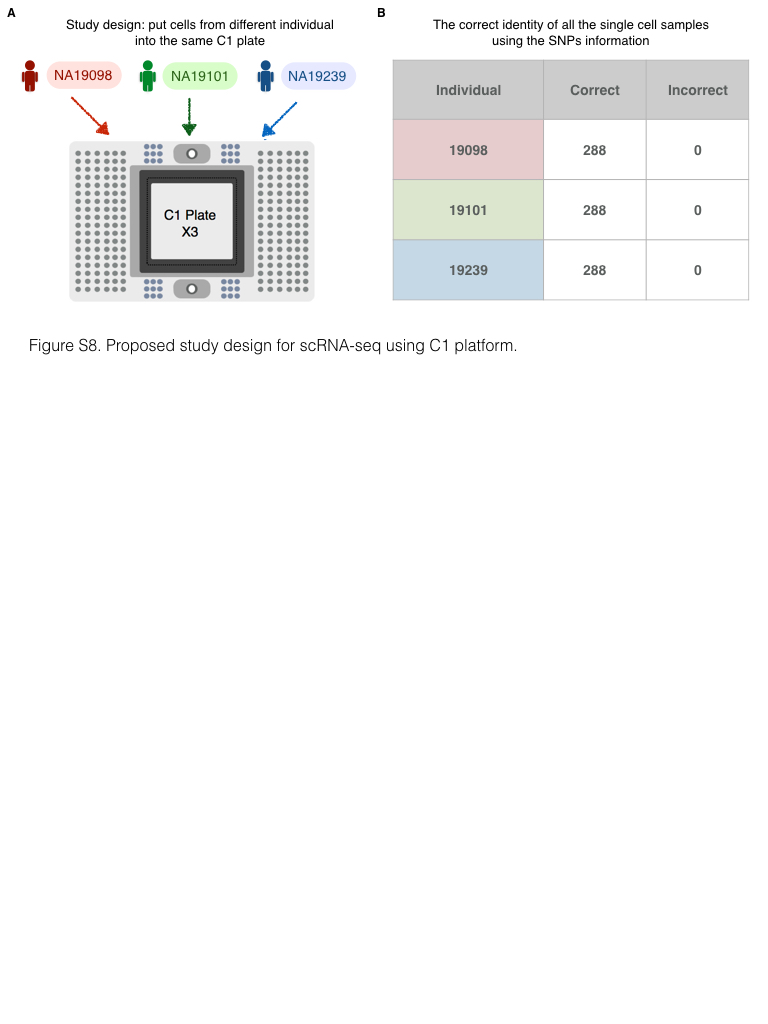
\includegraphics[trim=0 10in 0 0,clip,width=5in]{img/ch04/Figure13.jpeg}
\caption{\textbf{Supplementary Figure S8. Proposed study design for
scRNA-seq using C1 platform.} (A) A balanced study design consisting of
multiple individuals within a C1 plate and multiple C1 replicates to
fully capture the batch effect across C1 plates and further retrieve the
maximum amount of biological information. (B) The correct identity of
each single cell sample was determined by examining the SNPs present in
their RNA sequencing reads.}
\end{figure}

\begin{figure}[htbp]
\centering
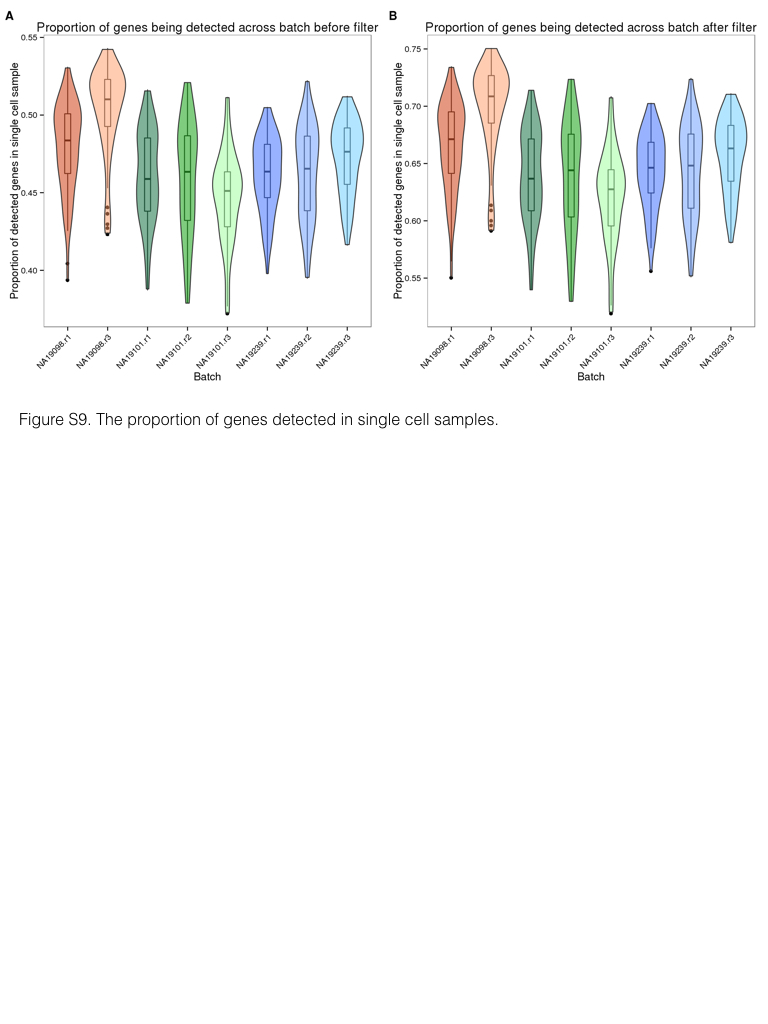
\includegraphics[trim=0 8.5in 0 0,clip,width=5in]{img/ch04/Figure14.jpeg}
\caption{\textbf{Supplementary Figure S9. The proportion of genes
detected in single cell samples.} Violin plots of the proportion of
genes detected, computed by the total number of detected genes in each
single cell divided by the total number of genes detected across all
single cells, before in (A) and after in (B) the removal of genes with
low expression. The three colors represent the three individuals
(NA19098 is in red, NA19101 in green, and NA19239 in blue).}
\end{figure}

\begin{figure}[htbp]
\centering
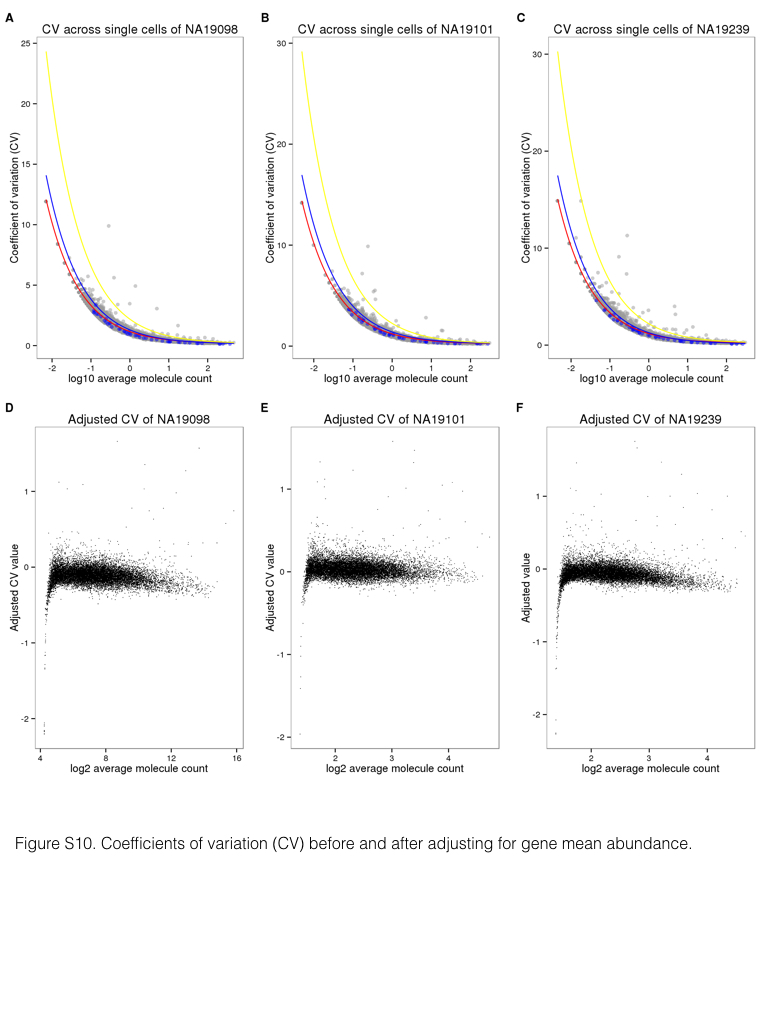
\includegraphics[trim=0 3in 0 0,clip,width=5in]{img/ch04/Figure15.jpeg}
\caption{\textbf{Supplementary Figure S10. Coefficients of variation
(CV) before and after adjusting for gene mean abundance.} (A-C) CV
plotted against average molecule counts across all cells for each
individual \citep{Islam2014}. Grey points represent endogenous genes, and
blue points represent ERCC spike-in controls. The curves indicate the
expected CV under three different scenarios. Red curve depicts the
expected CV of the endogenous genes while assuming a Poisson
distribution with no over-dispersion. Likewise, blue curve depicts the
expected CVs of the ERCC spike-in controls under the Poisson assumption.
Yellow curve depicts the expected CVs of an over-dispersed Poisson
distribution for which standard deviation is three times the ERCC
spike-in controls. (D-F) Adjusted CV values of each gene including all
cells are plotted against log\textsubscript{10} of the average molecule
counts for each individual.}
\end{figure}

\clearpage
\section{Supplementary Tables}\label{supplementary-tables}

\subsection{Supplementary Table S1. Data
collection.}\label{supplementary-table-s1.-data-collection.}

(A) iPSCs were sorted using the 10-17 $\mu$m IFC plates with the
staining of the pluripotency marker, TRA1-60. Single cell occupancy is
the percentage of occupied capture sites containing one single cell. The
average cDNA concentration was measured by the HT DNA high sensitivity
LabChip (Caliper). (B) The 96 single cell libraries from one C1 plate
were pooled and sequenced in three HiSeq lanes. The pooled samples were
assigned across the four 8-lane flowcells.

\begin{figure}[htbp]
\centering
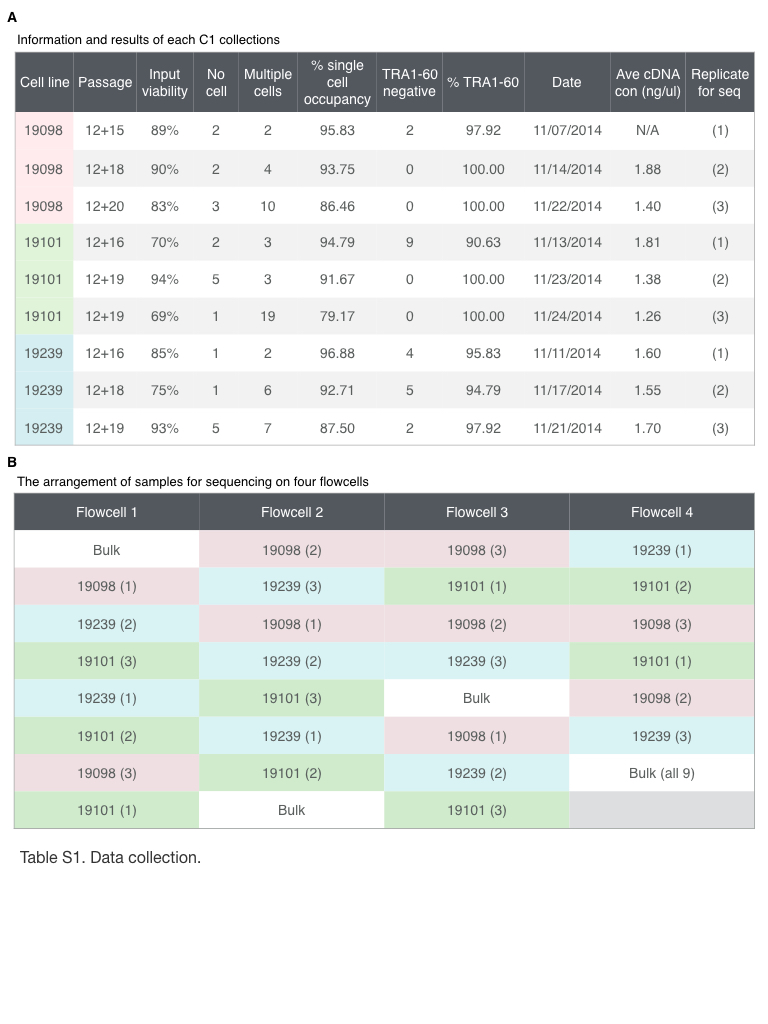
\includegraphics[trim=0 2.5in 0 0,clip,width=5in]{img/ch04/Figure16.jpeg}
\end{figure}
\clearpage

\subsection{Supplementary Table S2. High quality single cell
samples.}\label{supplementary-table-s2.-high-quality-single-cell-samples.}

List of the 564 high quality single cell samples.

\subsection{Supplementary Table S3. Genes associated with
inter-individual differences in regulatory
noise.}\label{supplementary-table-s3.-genes-associated-with-inter-individual-differences-in-regulatory-noise.}

List of genes that we classified the estimates of regulatory noise as
significantly different across individuals (empirical permutation
\emph{P} \textless{} 10\textsuperscript{-4}). There are a total of 560
genes.

\subsection{Supplementary Table S4. Gene ontology analysis of the
genes associated with inter-individual differences in regulatory
noise.}\label{supplementary-table-s4.-gene-ontology-analysis-of-the-genes-associated-with-inter-individual-differences-in-regulatory-noise.}

